\documentclass[tikz,border=8pt]{standalone}
% Shared look for every TikZ diagram. Load with % Shared look for every TikZ diagram. Load with % Shared look for every TikZ diagram. Load with \input{../../tools/tikz-style.tex}
\usepackage[T1]{fontenc}
\usepackage{lmodern}
\renewcommand{\sfdefault}{lmr}  % diagrams use the same serif as the text
\usetikzlibrary{arrows.meta, positioning, shapes.geometric, calc, fit, backgrounds}
\definecolor{cblue}{HTML}{4C78A8}
\definecolor{corange}{HTML}{F58518}
\definecolor{cgreen}{HTML}{54A24B}
\definecolor{cred}{HTML}{E45756}
\definecolor{cpurple}{HTML}{B279A2}
\definecolor{cgrey}{HTML}{6B6B6B}
\tikzset{
  every picture/.style={font=\sffamily, line width=1.2pt},
  box/.style={draw=#1, fill=#1!12, rounded corners=4pt, align=center, inner sep=7pt, minimum height=1.1cm},
  box/.default=cgrey,
  arrow/.style={-{Stealth[length=3mm]}, draw=cgrey, line width=1.4pt},
  title/.style={font=\sffamily\bfseries\Large},
  note/.style={font=\sffamily\small, text=cgrey, align=center},
}
\AtBeginDocument{\hyphenpenalty=10000 \exhyphenpenalty=10000}

\usepackage[T1]{fontenc}
\usepackage{lmodern}
\renewcommand{\sfdefault}{lmr}  % diagrams use the same serif as the text
\usetikzlibrary{arrows.meta, positioning, shapes.geometric, calc, fit, backgrounds}
\definecolor{cblue}{HTML}{4C78A8}
\definecolor{corange}{HTML}{F58518}
\definecolor{cgreen}{HTML}{54A24B}
\definecolor{cred}{HTML}{E45756}
\definecolor{cpurple}{HTML}{B279A2}
\definecolor{cgrey}{HTML}{6B6B6B}
\tikzset{
  every picture/.style={font=\sffamily, line width=1.2pt},
  box/.style={draw=#1, fill=#1!12, rounded corners=4pt, align=center, inner sep=7pt, minimum height=1.1cm},
  box/.default=cgrey,
  arrow/.style={-{Stealth[length=3mm]}, draw=cgrey, line width=1.4pt},
  title/.style={font=\sffamily\bfseries\Large},
  note/.style={font=\sffamily\small, text=cgrey, align=center},
}
\AtBeginDocument{\hyphenpenalty=10000 \exhyphenpenalty=10000}

\usepackage[T1]{fontenc}
\usepackage{lmodern}
\renewcommand{\sfdefault}{lmr}  % diagrams use the same serif as the text
\usetikzlibrary{arrows.meta, positioning, shapes.geometric, calc, fit, backgrounds}
\definecolor{cblue}{HTML}{4C78A8}
\definecolor{corange}{HTML}{F58518}
\definecolor{cgreen}{HTML}{54A24B}
\definecolor{cred}{HTML}{E45756}
\definecolor{cpurple}{HTML}{B279A2}
\definecolor{cgrey}{HTML}{6B6B6B}
\tikzset{
  every picture/.style={font=\sffamily, line width=1.2pt},
  box/.style={draw=#1, fill=#1!12, rounded corners=4pt, align=center, inner sep=7pt, minimum height=1.1cm},
  box/.default=cgrey,
  arrow/.style={-{Stealth[length=3mm]}, draw=cgrey, line width=1.4pt},
  title/.style={font=\sffamily\bfseries\Large},
  note/.style={font=\sffamily\small, text=cgrey, align=center},
}
\AtBeginDocument{\hyphenpenalty=10000 \exhyphenpenalty=10000}

% The chord test. Left: f(w) = w^2 with a = -1, b = 3, theta = 0.5: curve value 1, chord value 5 (chord above, convex).
% Right: g(w) = w^4 - 4w^2 + w with a = -1.5, b = 1.5: curve value g(0) = 0, chord value -3.94 (curve above, non-convex).
% Heights are drawn at 0.42 of their value (s below).
\def\s{0.42}
\begin{document}
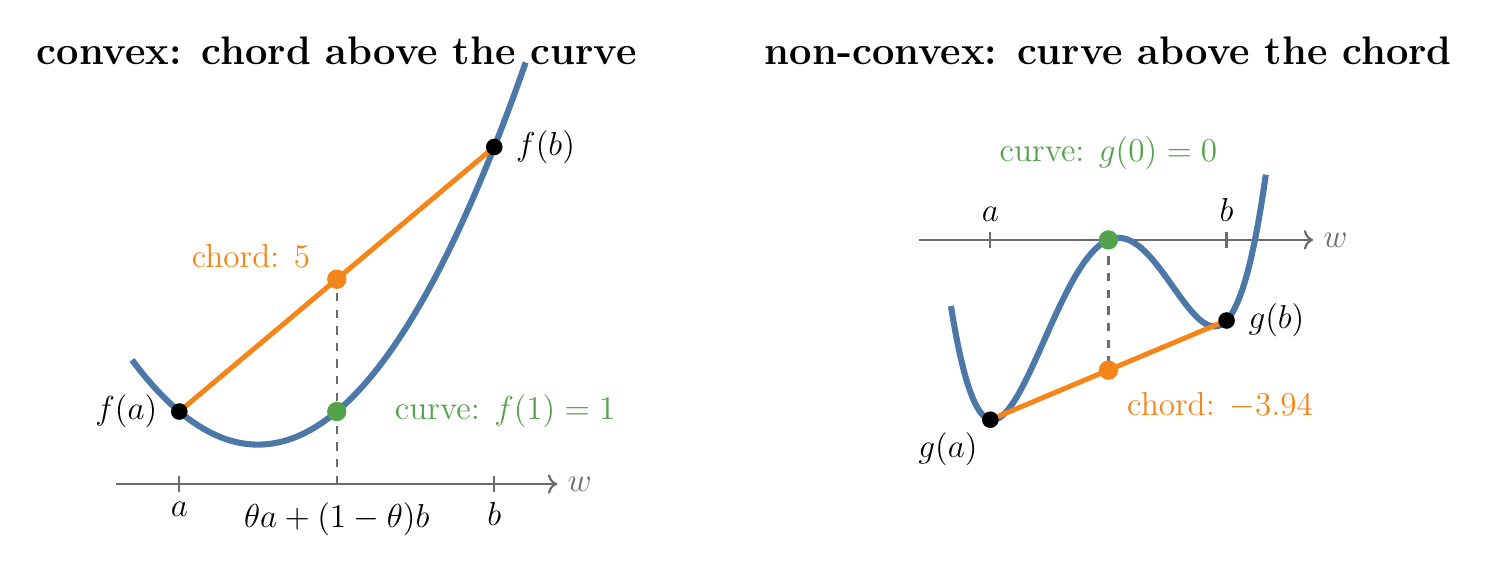
\begin{tikzpicture}[every node/.append style={font=\large}]
  % ---------- convex panel
  \draw[cgrey, line width=0.8pt, ->] (-1.8,-0.5) -- (3.8,-0.5) node[right] {$w$};
  \draw[cblue, line width=2.2pt] plot[domain=-1.6:3.4, samples=60, smooth] (\x, {\s*(\x)*(\x)});
  \draw[corange, line width=1.8pt] (-1,{\s*1}) -- (3,{\s*9});
  \fill (-1,{\s*1}) circle (3pt) node[left=4pt] {$f(a)$};
  \fill (3,{\s*9}) circle (3pt) node[right=4pt] {$f(b)$};
  \draw[cgrey, dashed, line width=0.9pt] (1,-0.5) -- (1,{\s*5});
  \fill[cgreen] (1,{\s*1}) circle (3.5pt);
  \fill[corange] (1,{\s*5}) circle (3.5pt);
  \node[cgreen, anchor=west] at (1.6,{\s*1}) {curve: $f(1) = 1$};
  \node[corange, anchor=east] at (0.8,{\s*5+0.3}) {chord: $5$};
  \foreach \p/\l in {-1/a, 3/b} \draw[cgrey, line width=0.8pt] (\p,-0.4) -- (\p,-0.6) node[below, black] {$\l$};
  \node[below] at (1,-0.6) {$\theta a + (1-\theta) b$};
  \node[title] at (1,5.0) {convex: chord above the curve};
  % ---------- non-convex panel
  \begin{scope}[xshift=10.8cm, yshift=2.6cm]
    \draw[cgrey, line width=0.8pt, ->] (-2.4,0) -- (2.6,0) node[right] {$w$};
    \draw[cblue, line width=2.2pt] plot[domain=-2.0:2.0, samples=120, smooth] (\x, {\s*((\x)^4 - 4*(\x)^2 + \x)});
    \draw[corange, line width=1.8pt] (-1.5,{\s*-5.4375}) -- (1.5,{\s*-2.4375});
    \fill (-1.5,{\s*-5.4375}) circle (3pt) node[below left=1pt] {$g(a)$};
    \fill (1.5,{\s*-2.4375}) circle (3pt) node[right=4pt] {$g(b)$};
    \draw[cgrey, dashed, line width=0.9pt] (0,0) -- (0,{\s*-3.94});
    \fill[cgreen] (0,0) circle (3.5pt);
    \fill[corange] (0,{\s*-3.94}) circle (3.5pt);
    \node[cgreen, anchor=south] at (0,0.75) {curve: $g(0) = 0$};
    \node[corange, anchor=north west] at (0.1,{\s*-3.94-0.15}) {chord: $-3.94$};
    \foreach \p/\l in {-1.5/a, 1.5/b} \draw[cgrey, line width=0.8pt] (\p,0.1) -- (\p,-0.1);
    \node[above] at (-1.5,0.1) {$a$}; \node[above] at (1.5,0.1) {$b$};
    \node[title] at (0,2.4) {non-convex: curve above the chord};
  \end{scope}
\end{tikzpicture}
\end{document}
